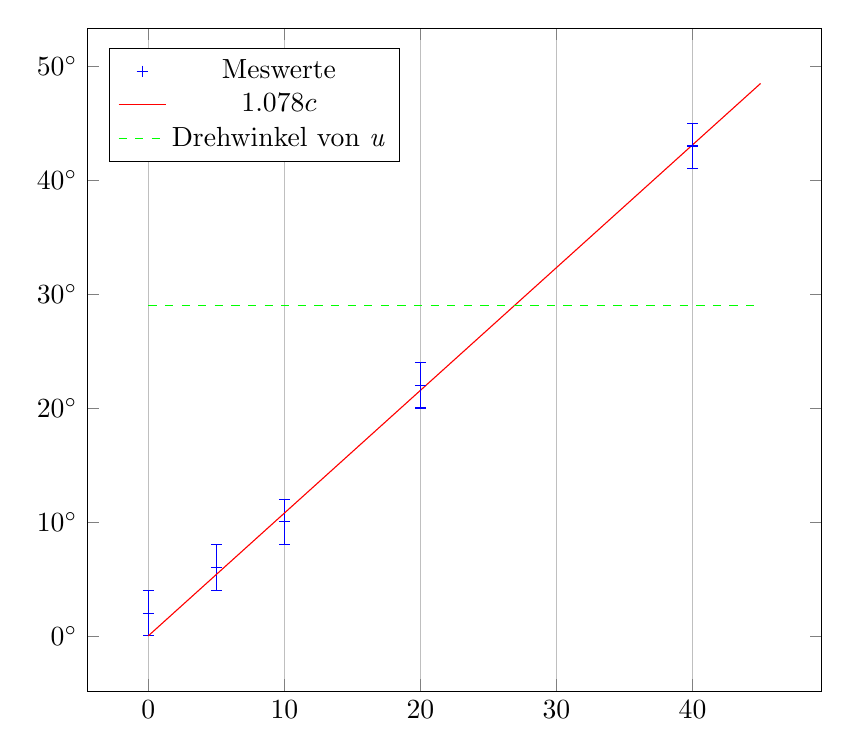
\begin{tikzpicture}
\begin{axis}[yticklabel=$\pgfmathprintnumber{\tick}^\circ$, width=.9\linewidth, height=10cm,
	legend pos = north west, xmajorgrids]
	\addplot+ [only marks, mark=+, 
		error bars/.cd,
		y dir = both, y fixed = 2] 
	table[x=x,y=y] {
x	y
0	2
5	6
10	10
20	22
40	43
	};
	\addplot+[domain= 0:45, no marks] {1.07764705830693*x};
	\addplot+[domain=0:45, no marks, green, dashed] {29};
\legend{Meswerte, $ \num{1.078 }c $, Drehwinkel von \textit{u}}
\end{axis}

\end{tikzpicture}